\RequirePackage[l2tabu, orthodox]{nag}
\documentclass[a4paper,12pt, openright, twoside]{report}
\usepackage{listings}
\usepackage{color} %red, green, blue, yellow, cyan, magenta, black, white
\usepackage[T1]{fontenc}
\usepackage[utf8]{inputenc}
\usepackage[american]{babel}
\usepackage[breaklinks=true,colorlinks=false,pdfborder={0 0 0}]{hyperref}
\usepackage{lmodern}
\usepackage{graphicx}
\usepackage{datetime2}
\usepackage{url}
%\usepackage{breakurl}
\usepackage{wrapfig}
\usepackage{subcaption}
\usepackage{microtype}
%\usepackage{inconsolata}
%\usepackage[lf]{MinionPro}
\usepackage{textcomp}
\usepackage{booktabs}
\usepackage{multirow}
\usepackage{amsmath}
\usepackage{cleveref}
\usepackage{courier}
\usepackage{xstring}
\usepackage{mathrsfs}
\usepackage{units}
\usepackage{threeparttable}
\usepackage{enumitem}
\usepackage{todonotes}
\usepackage{gensymb}
\usepackage{lipsum}
\usepackage{fancyhdr}
\usepackage[headsep=.5cm,headheight=1cm,left=3cm,right=2cm,top=3cm,bottom=2.5cm]{geometry}
\usepackage[numbib]{tocbibind}
\usepackage{appendix}
\usepackage{imakeidx}


\makeindex
\indexsetup{level=\section,noclearpage}

\reversemarginpar
\setlength{\marginparwidth}{2cm}

\providecommand{\keywords}[1]{\textbf{\textit{Keywords: }} #1}
\def\UrlBreaks{\do\/\do-}
\definecolor{mygreen}{RGB}{28,172,0} % color values Red, Green, Blue
\definecolor{mylilas}{RGB}{170,55,241}


\lstset{language=Matlab,%
    basicstyle=\footnotesize\ttfamily,
    %basicstyle=\color{red},
    flexiblecolumns=true,
    breaklines=true,%
    morekeywords={matlab2tikz,tf,series,parallel,feedback},
    keywordstyle=\color{blue},%
    morekeywords=[2]{1}, keywordstyle=[2]{\color{black}},
    identifierstyle=\color{black},%
    stringstyle=\color{mylilas},
    commentstyle=\color{mygreen},%
    showstringspaces=false,%without this there will be a symbol in the places where there is a space
    numbers=left,%
    numberstyle={\tiny \color{black}},% size of the numbers
    numbersep=9pt, % this defines how far the numbers are from the text
    emph=[1]{for,end,break},emphstyle=[1]\color{red}, %some words to emphasise
    %emph=[2]{word1,word2}, emphstyle=[2]{style},    
}



\title{Agricultural Field Detection and Path Planning for an Unmanned Aerial Vehicle}
\author{Michael Rimondi}
\date{\today}


% Make the list of * output as SECTION rather than CHAPTER
\makeatletter
\newcommand\renewlistof[3]%
   {\renewcommand#1%
      {\section{#3}%
       %\addcontentsline{toc}{chapter}{#3}%
       \markboth{#3}{#3}%
       \@starttoc{#2}%
      }%
   }
\makeatother
\renewlistof\listoffigures{lof}{\listfigurename}
\renewlistof\listoftables{lot}{\listtablename}
\renewlistof\lstlistoflistings{lstlol}{\lstlistlistingname}

%!TEX root = bambi-thesis.tex

\def\maketitle{\begingroup % Create the command for including the title page in the document
% \centering % Center all text
% \thispagestyle{empty} 
% \vspace*{4cm}

% \rule{\textwidth}{1.6pt}\vspace*{-\baselineskip}\vspace*{2pt} % Thick horizontal line
% \rule{\textwidth}{0.4pt}\\[\baselineskip] % Thin horizontal line

% {\LARGE  \textsc{\@title}}\\[0.2\baselineskip] % Title

% \rule{\textwidth}{0.4pt}\vspace*{-\baselineskip}\vspace{3.2pt} % Thin horizontal line
% \rule{\textwidth}{1.6pt}\\[\baselineskip] % Thick horizontal line

% \scshape % Small caps
% \subtitle\\[1.5\baselineskip] % Tagline(s) or further description
% Bologna, \@date \par % Location and year

% \vspace*{2\baselineskip} % Whitespace between location/year and editors

% \subject

% \vspace*{2\baselineskip} % Whitespace between location/year and editors

% Edited by \\[\baselineskip]
% {\Large \@author\\[2\baselineskip]\par} % Editor list
% \includegraphics[width=.15\textwidth]{figures/universitiy-of-bologna-logo.jpg}\\[0.3\baselineskip]
% {\itshape Università di Bologna\par} % Editor affiliation
% \vfill % Whitespace between editor names and publisher logo



% \vspace*{\baselineskip} % Whitespace between location/year and editors

% \textit{\textbf{Supervisors:}\\[\baselineskip]\textsc{\mentors}}

\thispagestyle{empty} 
\begin{center}
{{\Large{\textsc{Alma Mater Studiorum $\cdot$ Università di
Bologna}}}}\\
\vskip - 5pt
\rule{\textwidth}{0.1mm}
\rule[0.5cm]{\textwidth}{0.6mm}
\vskip -13pt
{\small{\textsc{Scuola di Ingegneria e Architettura\\
\vspace{4mm}
\small{Dipartimento di Ingegneria dell'Energia Elettrica e dell'Informazione \\
"Guglielmo Marconi" – DEI\\}}}}
% 
% 
% SCUOLA DI INGEGNERIA E ARCHITETTURA
% DIPARTIMENTO DI
% INGEGNERIA DELL'ENERGIA ELETTRICA E DELL'INFORMAZIONE
% "Guglielmo Marconi"
% DEI
% 
\vspace{15mm}
{\large{\textsc{{Corso di Laurea in Ingegneria dell'Automazione}}}}
\vskip 5mm
\rule{10cm}{0.4mm}
\rule[0.5cm]{10cm}{0.1mm}\\
\vskip -5pt
{\LARGE\textbf{{Agricultural Field Detection}}}\\
\vspace{.5em}
{\LARGE{\textbf{{and Path Planning}}}}\\
\vspace{.5em}
{\LARGE{\textbf{{for an Unmanned Aerial Vehicle}}}}\\
%\vspace{3mm}
%{\LARGE{\textbf{ --}}}\\
\vskip -2pt
\rule{10cm}{0.1mm}
\rule[0.5cm]{10cm}{0.4mm}\\
\vspace{5mm} {\large{\textsc{Progetto di Laurea}}}
\end{center}
\vspace{8mm}
\centering

\includegraphics[width=.25\textwidth]{figures/university-of-bologna.pdf}
\vfill
\par
\noindent
\begin{minipage}[t]{0.47\textwidth}
{\large{\textit{Relatore:}}\\
{\textbf{Chiar.mo Prof. Lorenzo Marconi}}}\\
\vskip 8pt
{\large{\textit{Correlatore:}}\\
{\textbf{Prof. Nicola Mimmo}}}
\end{minipage}
\hfill
\begin{minipage}[t]{0.47\textwidth}\raggedleft
{\large{\textit{Presentato da:}}\\
%\vspace{2mm}
{\textbf{Michael Rimondi}}}
\end{minipage}
\vspace{22mm}
\begin{center}
{\large{\textsc{II Sessione\\%inserire il numero della sessione in cui ci si laurea
Anno Accademico 2017/2018}}}%inserire l'anno accademico a cui si è iscritti
\end{center}



\newpage

\endgroup}
\makeatother


% clear fancy hdr spaces
\fancyhf{}
\renewcommand*{\sectionmark}[1]{ \markright{\thesection\ ##1} }
\fancyhead[LE,RO]{\rightmark}
\fancyhead[LO,RE]{\leftmark}
\fancyfoot[C]{\thepage}
\pagestyle{fancy}

\begin{document}


\hypersetup{pageanchor=false}
\maketitle

%%%%%%%%%%%%%% REMOVE ME %%%%%%%%%%%%%%%%%
\thispagestyle{empty}
\listoftodos
\pagenumbering{roman}
\setcounter{page}{1}
\newpage
%%%%%%%%%%%%%% REMOVE ME %%%%%%%%%%%%%%%%%

\thispagestyle{empty}
\setcounter{page}{2}
\cleardoublepage


\pagenumbering{roman}
\begin{abstract}
\addcontentsline{toc}{chapter}{Abstract}{}{}
\thispagestyle{plain}
\setcounter{page}{3}
\lipsum[43]
\vskip 2em
\keywords{One, Two}
\end{abstract}

\thispagestyle{empty}
\setcounter{page}{4}
\cleardoublepage


\renewcommand{\abstractname}{Abstract (italiano)}
\begin{abstract}
\addcontentsline{toc}{chapter}{Abstract (italiano)}{}{}
\thispagestyle{plain}
\setcounter{page}{5}
\lipsum[44]
\vskip 2em
\keywords{Uno, Due}
\end{abstract}



\thispagestyle{empty}
\cleardoublepage

% use pagestyle plain for content to put page numbers in the footer
\hypersetup{pageanchor=true}
\pagestyle{plain}
\tableofcontents

\cleardoublepage


% begin content and use roman numbers for chapter,
% without including them in the section numbering (no I.1)
\pagestyle{fancy}
\pagenumbering{arabic}
\renewcommand{\thechapter}{\Roman{chapter}}
\renewcommand*\thesection{\arabic{section}}


\chapter{Introduction} % (fold)
\label{cha:introduction}

%!TEX root = bambi-thesis.tex



In this introduction it is first briefly described the motivation, objective and scope of the project this thesis has been developed in. Once the background has been well set and explained,it will be describe the specific subject of the thesis.


\section{Motivation} % (fold)
\label{sec:motivation}
 Deers gives birth to their offspring during April and May \cite{MowlingMortality}, often choosing meadows as they consider it a safe spot. This period is unfortunately the same in which meadows are cut. The results is that every year a great number of young deers fall victim of combine harvesters cutting hay. Germany counts about 100000 death every harvest season \cite{MowlingMortality}.
 The BambiSaver project was born aiming to provide an autonomous, fast and user friendly device able to search and locate, living creatures in agricultural areas. It is, as a matter of fact, difficult to locate small animals hidden in vast grasslands especially if they freeze when they feel under threat. For this specific reason the proposal design is based on a UAV (Unmanned Aerial Vehicle) \cite{ICAO} and more precisely a quad-copter equipped with a thermal camera.
 An aerial vehicle is, in fact, able to efficiently cover large surfaces way faster then any other ground alternatives and guarantees the best viewpoint for the specific kind of wildlife research. Moreover it has been chosen a copter rather than a fixed wing model for its holonomic properties which turns out to be very useful in upland regions as well as for small and irregular fields. It is basically why in search and rescue operations helicopters are often adopted instead of planes.

\subsection{Importance for Wildlife and for Agricultural}
\index{Agriculture}
In early hunting literature from as far back as the mid-19th century, references can be found to significant losses of breeding partridges and pheasants from the use of sickle and scythe. Due to the fierce competition in the agricultural sector, developments in agricultural technology have brought about a tremendous acceleration in mowing techniques, with tendency still rising. Today, mowing speed can even exceed 15 km/h, while at the same time ever-wider mowers are used. Nesting birds, young hares and fawns are regular victims of such mowers and even full-grown wild animals cannot always escape. Ever since the 1950s, the importance of silage meadows has increasingly taken precedence over the traditional hay harvest.

\subsection{Affected Species} % (fold)
\label{sub:affected_species}
Grassland is used by countless species of wildlife as food, cover and reproduction habitat. Apart from leverets, fawns and various field birds, small mammals, amphibians and insects all fall victim to the practice of early and more frequent mowing. Formerly reliable survival strategies proven successful over thousands of years have a devastating effect in mowing situations. The instinct of the brooding partridge hen to sit tight on her nest, or of the hare or fawn to freeze motionless, now prove fatal. The optimized patterns of predator avoidance behavior which wild animals have evolved can no longer keep up with the developments in modern cultivation techniques.
% subsection affected_species (end)
5de0697a03
\subsection{Measure to Reduce Wildlife Losses} % (fold)
\label{sub:measure_to_reduce_wildlife_losses}
 The most important factor influencing wildlife mortality is without doubt the time of mowing. On the other hand, economic considerations make this a crucial factor for the farmer, too. A late mowing is good for wildlife but not ideal for the farmer from the point of view of yield and quality. Yet there are some other factors in the mowing of arable land which offer potential for reducing wildlife losses \cite{MowlingMortality}:
\begin{itemize}
	\item \textit{Cutting height}: the higher the cut, the lower will be the losses suffered by crouching animals and nesting birds.
	\item \textit{Mowing direction}: mowing the field from the center outwards gives fully-grown wild animals the opportunity to escape.
	\item \textit{Mowing date}: late cuts,from mid-July onwards, reduce the losses to wildlife during the nesting and rearing period.
	\item \textit{Mowing strategy}: mowing of partial areas, leaving edge strips unmown.
	\item \textit{Mowing frequency}: a longer interval between first and second cuttings reduces the mortality rate, especially for ground-nesting birds.
	\item \textit{Mowing technology}: cutter-bar mowers cause less harm to wild animals than rotary mowers.
\end{itemize}
 Another practical approach is the one adopted in a German wildlife rescue project which consists in deploying small aerial drones to find young deer hiding in tall grass.
% subsection measure_to_reduce_wildlife_losses (end)

\section{State of the art} % (fold)
\label{sec:state_of_the_art}
 During last years, the increasing interest and development of UAS (Unmanned Aircraft System) makes them affordable and suitable for many different applications. Specifically, in wildlife research, drones are frequently use as they are less expensive, quieter, and safer than traditional manned aircraft. Most studies we reviewed recorded minimal or no visible behavioral responses to UAS; however, UAS are capable of causing behavioral and physiological responses in wildlife when observing at close range. \cite{doi:10.1002/fee.1281}.\\
 For the case under-study, the "Flying Wildlife Finder", represents the state-of-the-art.
 The project, developed by the German Aerospace Center (DLR), is an application system which prevents accidents by detecting animals hidden in tall grass during the hay harvest. 
 The "Flying Wildlife Finder", a remotely controlled aerial drone equipped with sensors and a GPS link, is sent on a reconnaissance flight before mowing starts. A high resolution thermal imaging camera detects the temperature of animals hidden in the grass, which is higher than the ambient temperature of the field. Once the animal is located a search party is led to the fawn’s resting place with the help of GPS.
 This solution proves to be good as it is less time-consuming then using trained dog, while maintaining even higher "hit-rate", but it has the main drawback of requiring at least two specialists: one pilot and one camera operator that must be focused on the thermal video stream during the whole mission duration.

 
% section state_of_the_art (end)
 
 \section{Proposal Solution} % (fold)
 \label{sec:proposal_solution}
 In the following section it is briefly explained the goals and design guidelines of the project.
 % section proposal_solution (end)

 \subsection{Project Goals} % (fold)
 \label{sec:bambisaver_goals}
 The scope of BambiSaver is to design an integrated system capable to autonomously handle every steps of the mission so that it can be operated also by untrained personals. This must be guaranteed even in adverse environments, especially in uneven fields as it is in upland regions. \todo{????the idea was developed having the mountain of Trentino Altoadige in mind????}
 Along with this, it is of particular interest to keep modularity in every hardware and software components. This is to permit easier implementation of new features or improvements.
 All this guidelines \todo{sinonimo per dire idee alla bass} have been taken into account during the design and implementation stages (i.e. ROS as framework for the on-board computer).

 \subsubsection{Software Design concept} % (fold)
 \label{ssub:software_design}
 The raspberry Pi 3 it is used as on-board computer, it runs ROS and manages the transition between the different mission's phases. The software develops according to the usual ROS philosophy \cite{288}, thus it is composed of five nodes implementing every mission component as an independent module. \autoref{fig:rqtgraph} displays all the nodes and the related topics used to let them communicate.
\begin{figure}[ht]
    \centering
    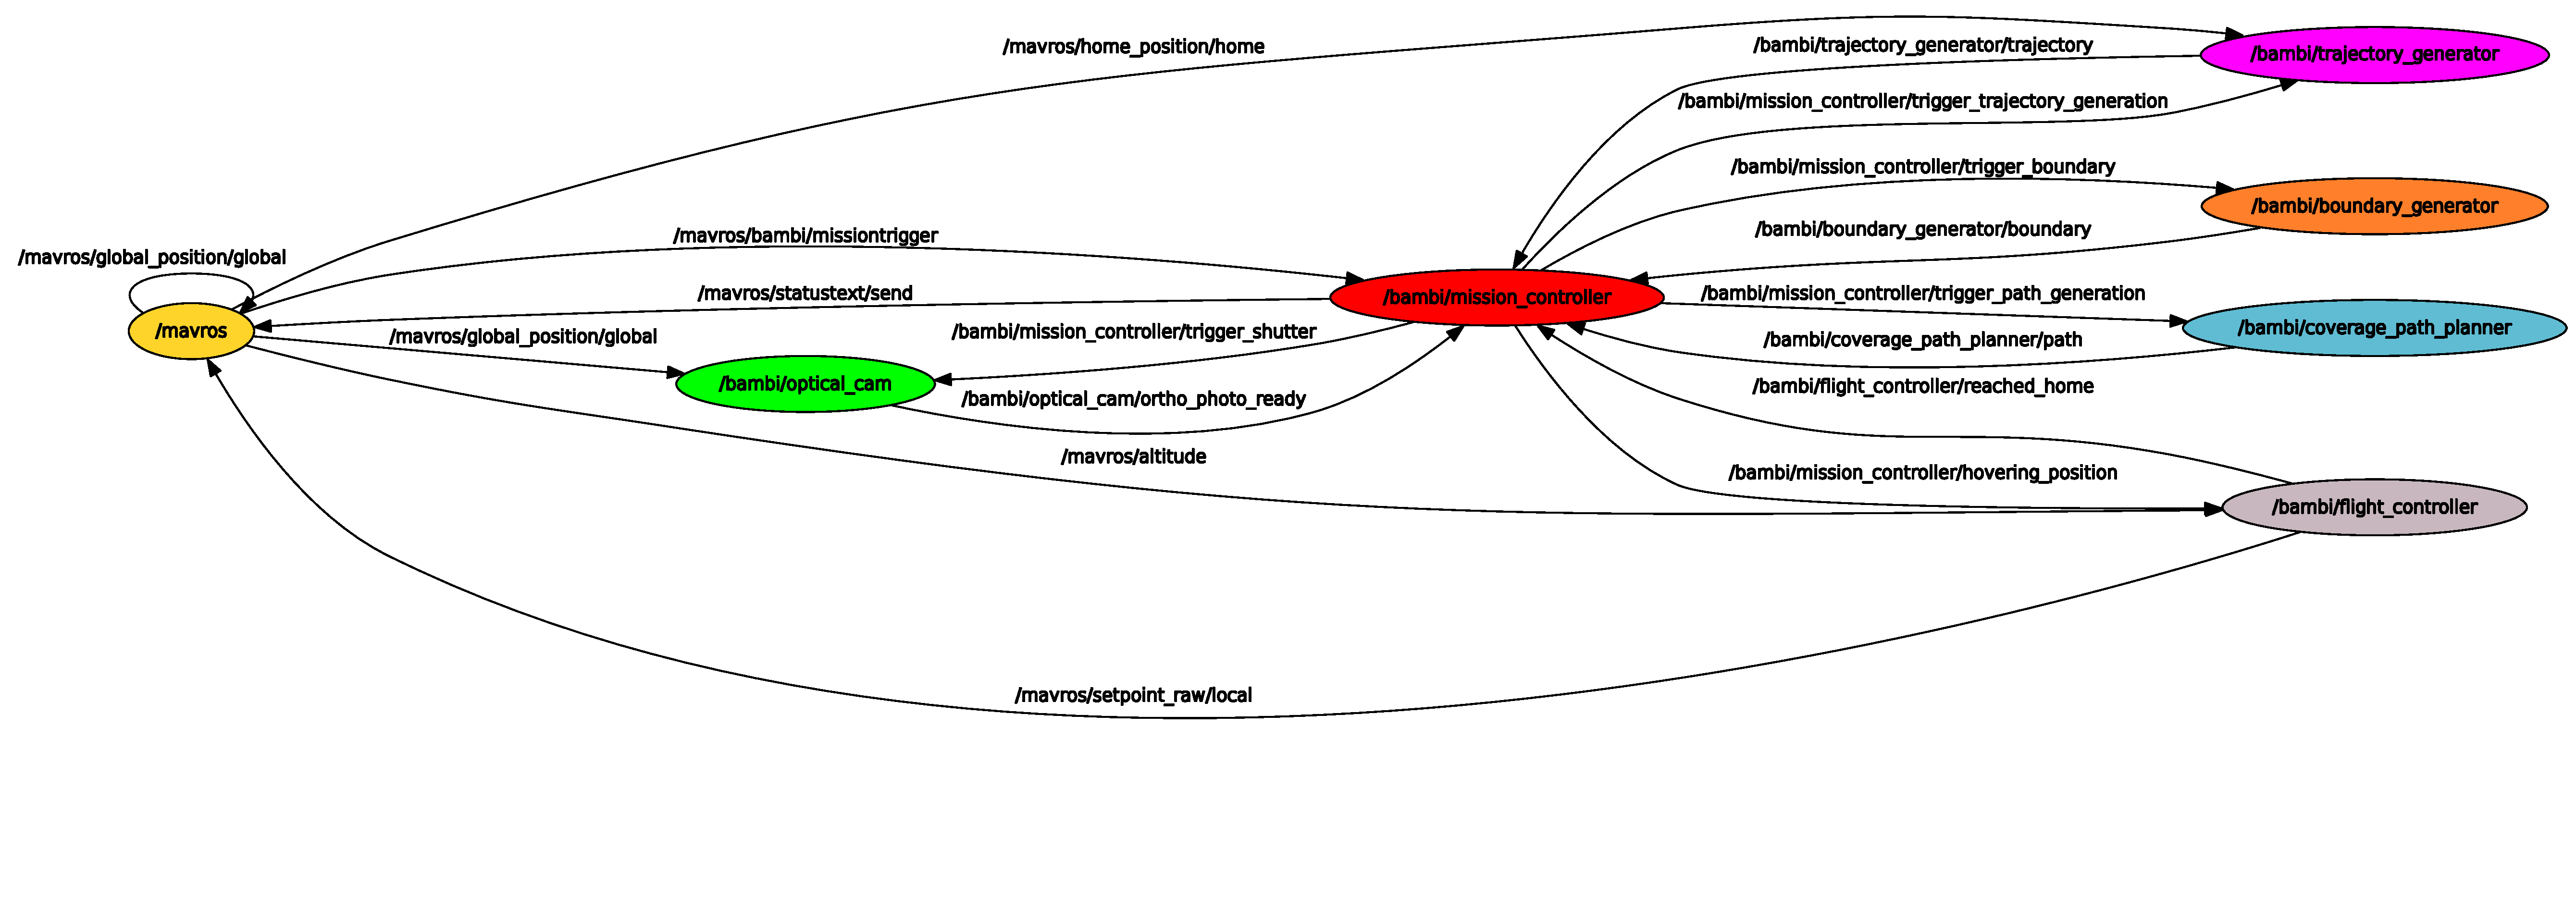
\includegraphics[width=1.4\textwidth, angle=270]{figures/C1/rqtgraph.eps}
    \caption{Nodes and Topics graph}
    \label{fig:rqtgraph}
\end{figure}\\
 In the following chapter the thesis will focus, exclusively on two problems:
 \begin{itemize}
  	\item \textit{Geo-referencing the mission's environment and get the field boundary}. This is of great importance, as it define the mission's range which is fundamental for every successive tasks.
  	\item \textit{Planning the coverage path}.It regards planning the geometric path so that the whole field of interest is covered by the sensor footprint.
  \end{itemize}
 
  % subsubsection software_design (end)

 

{}

 % Da mettere nel corpo della tesi NON INTRO
 % section bambisaver_goals (end)
% \section{Hardware Setup} % (fold)
% \label{sec:hardware_setup}
% The quadcopter (UAV) is equipped with:
% \begin{itemize}
% 	\item Pixhawk flashed with PX4 flight stack (see appendix \ref{appendix:pixhawk_flight_controller})
% 	\item NEO-M8n (GPS){}
% 	\item 3DR telemetry radio 433Hz (serial link between the UAV and the ground station)
% 	\item LidarLite V3 (altitude distance sensor) \cite{grm:lidarlite}
% 	\item Raspberry Pi 3b (Onboard computer running ROS over Ubuntu OS)
% \end{itemize} 
%  The ground station is composed by a common laptop running QGroundControl \todo{appendix or small description and features of QGC} application. The communication with the UAV uses the MAVLink protocol \cite{Mavlink} through an USB 433Hz telemetry radio .
% % section hardware_setup (end)

% \section{Software} % (fold)
% \label{sec:software}

% \todo{ROS, PX4 why we choose them}
% \todo{ROS design graph and explanation of each node}
% \todo{go deeply in ortho photo a}
% % section software (end)
% section  (end)
\section{Innovation} % (fold)
\label{sec:innovation}
 
 The approach 
The proposal device is an UAV \cite{ICAO}


\begin{align}
  \vec F &= \vec a \times \vec b\\
  {dof}_{rot} &= \sum_{i=1}^n (i-1) = n\, \frac{n-1}{2}
\end{align}


% section innovation (end)

% chapter introduction (end)



\chapter{Georeferencing the mission's environment} % (fold)
\label{cha:georeferencing_the_mission_s_environment}

% chapter georeferencing_the_mission_s_environment (end)



\cleardoublepage
\pagestyle{plain}

\begin{appendices}

\bibliography{bambi-thesis}
\bibliographystyle{alpha}

\chapter{Supplementary Information} % (fold)
\label{cha:supplementary_information}


\listoffigures
\listoftables
\lstlistoflistings
\printindex

% chapter supplementary_information (end)


\end{appendices}

\end{document}
